\documentclass[10pt,xcolor=table ]{beamer}
	
\usetheme{metropolis}
\usepackage{appendixnumberbeamer}

\usepackage{booktabs}
\usepackage[scale=2]{ccicons}

\usepackage{pgfplots}
\usepgfplotslibrary{dateplot}

\usepackage{xspace}
\usepackage{graphicx}
\usepackage{graphics}


\usepackage[spanish]{babel}
\usepackage[utf8]{inputenc}

\usepackage{decorule}
\newcommand{\decoRule}{\rule{\textwidth}{.4pt}} % New command for a rule to be used under figures

\usepackage[export]{adjustbox}


\definecolor{UniBlue}{RGB}{255,255,255}
\setbeamercolor{background canvas}{bg=UniBlue}


\title{Desarrollo de un sistema de gestión de programas de estudio orientado a resultados pedagógicos}
\subtitle{Proyecto final de la carrera}
\date{\today}
\author{Luis Fernando Villalba Vera}
\institute{Universidad Católica - Nuestra Señora de la Asunción}
% \titlegraphic{\hfill\includegraphics[height=1.5cm]{logo.pdf}}

\begin{document}

\maketitle

\begin{frame}{Contenido}
	\begin{enumerate}
	    \item Problemática y justificación
	    \item Objetivos
	    \item Estado del arte
	    \item Caso de estudio
	    \item Propuesta de trabajo
	    \item Proceso de desarrollo
	    \item Validación
	    \item Conclusión y aportes
	 \end{enumerate}
\end{frame}
% PROBLEMÁTICA Y JUSTIFICACIÓN
\section{Problemática y Justificación}
\begin{frame}{Conceptos}
  \begin{itemize}[<+- | alert@+>]
    \item Problemática.
    \item Competencias académicas y su evaluación.
    \item Sistemas de gestión de evaluaciones (AMS).
    \item Sistemas de gestión curricular (CMS)
  \end{itemize}
\end{frame}

% Diseño de programas
\subsection{Diseño de cursos y programas}
\begin{frame}{Diseño de cursos y programas}
	\begin{figure}
		\centering
	    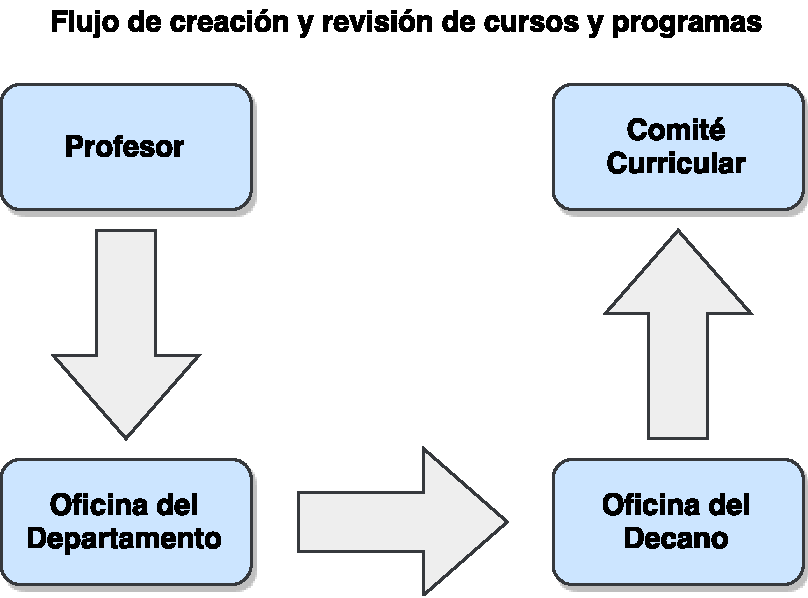
\includegraphics[scale=0.6]{../Figuras/problematica/flujo_autoridades}
	\end{figure}
\end{frame}

% Estándares de California
\subsection{Estándar de cursos y programas}
\begin{frame}{Estándar de cursos y programas}
  	\metroset{block=fill}
	\begin{alertblock}{Definición}
		Patrón de definición de cursos y programas para el estado de California.
	\end{alertblock}

	\begin{columns}[c,onlytextwidth]
    	\column{0.6\textwidth}
		\begin{block}{Provee}
			\begin{itemize}
				\item Definiciones de cursos y programas.
				\item Taxonomía de programas.
				\item Flujo para revisión de cursos y programas existentes.
				\item Guía de desarrollo de propuestas
				\item Establecido por el PCAH[1].
			\end{itemize}
		\end{block}
	    \column{0.4\textwidth}
		\begin{figure}
		    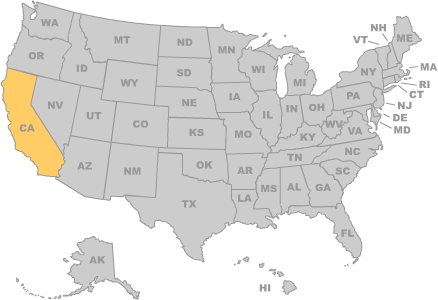
\includegraphics[scale=0.25]{../Figuras/usmap-ca}
		\end{figure}
  	\end{columns}
  	\decoRule \\
  \tiny [1] \textit{Brice W. Harris. Program and Course Approval Handbook. English. Fifth Edition. Sept. 2013.} \\
\end{frame}
\subsection{Diseño de cursos y programas}
\begin{frame}{Diseño de cursos y programas}
	\begin{figure}
		\centering
	    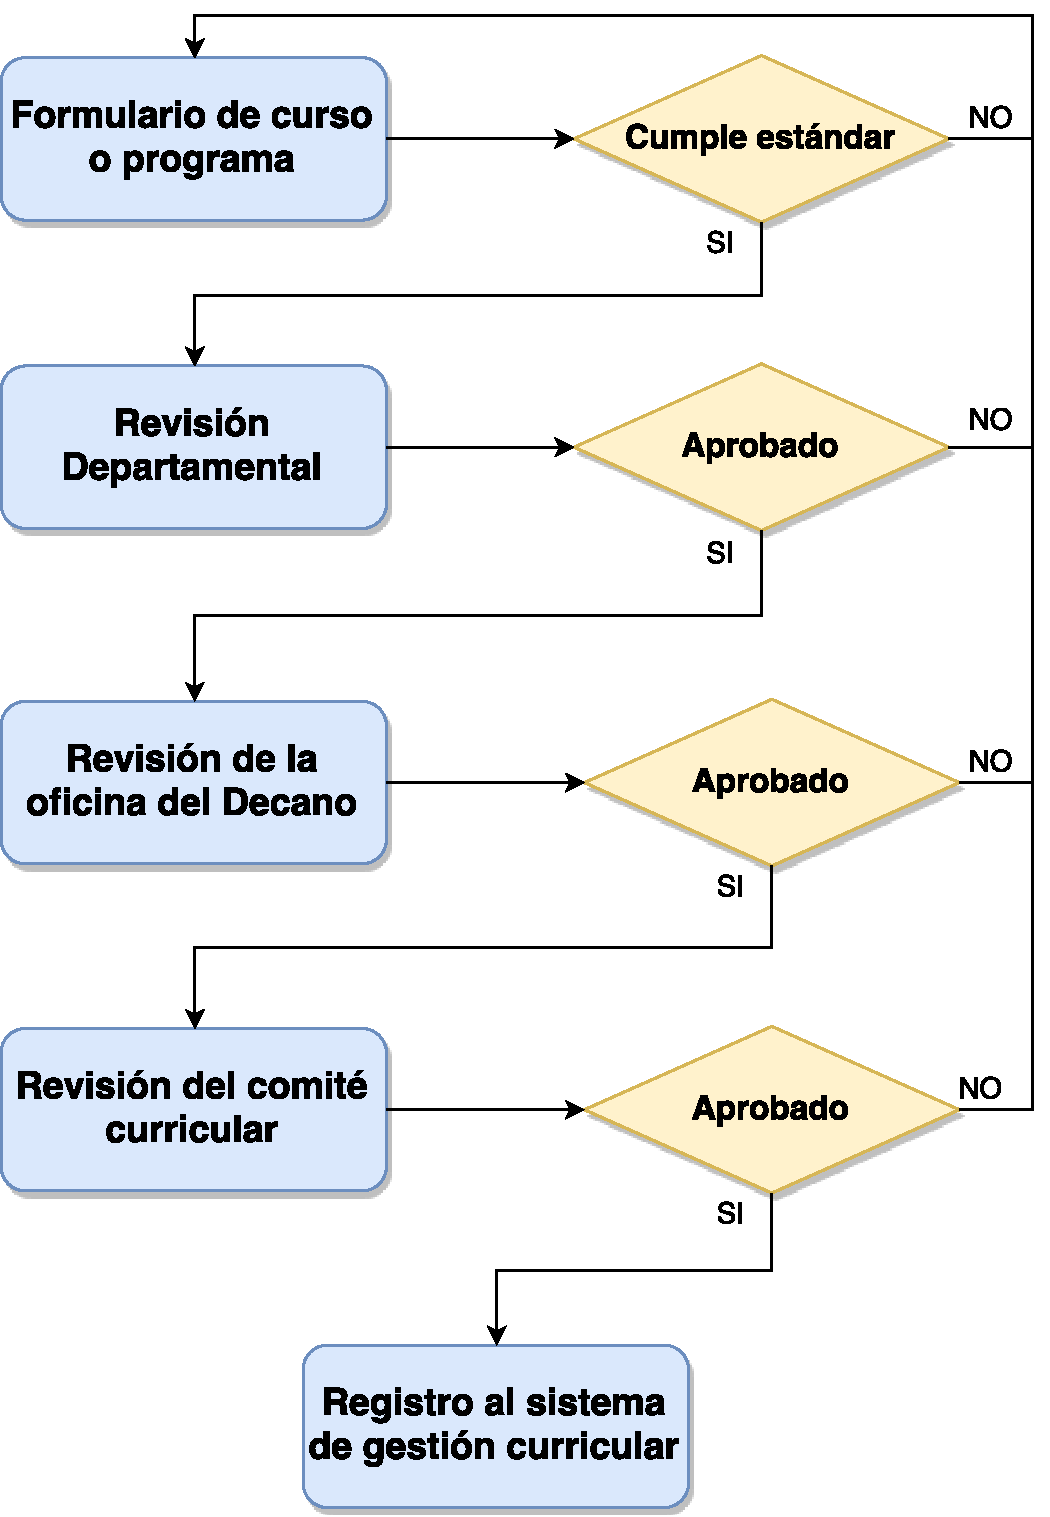
\includegraphics[scale=0.3]{../Figuras/problematica/course_creation_flow}
	\end{figure}
\end{frame}

\subsection{Disponibilidad en el sistema de gestión de competencias}
\begin{frame}{Disponibilidad en el sistema de gestión de competencias}
	\begin{figure}
		\centering
	    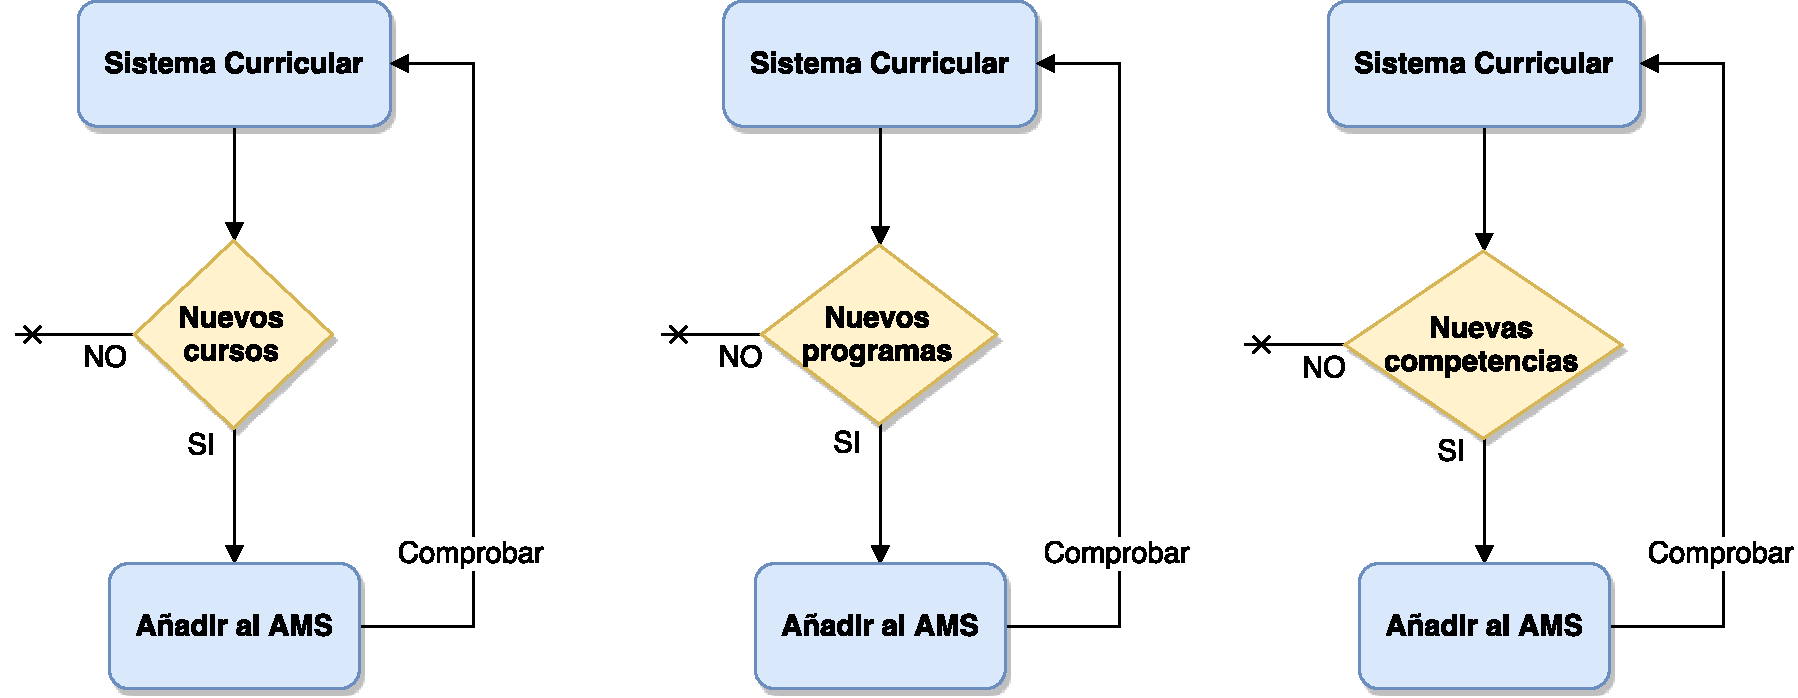
\includegraphics[scale=0.35]{../Figuras/problematica/after_creation}
	\end{figure}
\end{frame}


\subsection{Sistemas de gestión curricular}
\begin{frame}{Sistemas de gestión curricular}
	\begin{figure}
		\centering
	    
\includegraphics[scale=0.5]{../Figuras/problematica/cms_alternatives}
	\end{figure}
\end{frame}

% Facil e intuitivo
\subsection{Experiencia de usuario}
\begin{frame}{Experiencia de usuario}
	\begin{figure}[H]
			\centering
			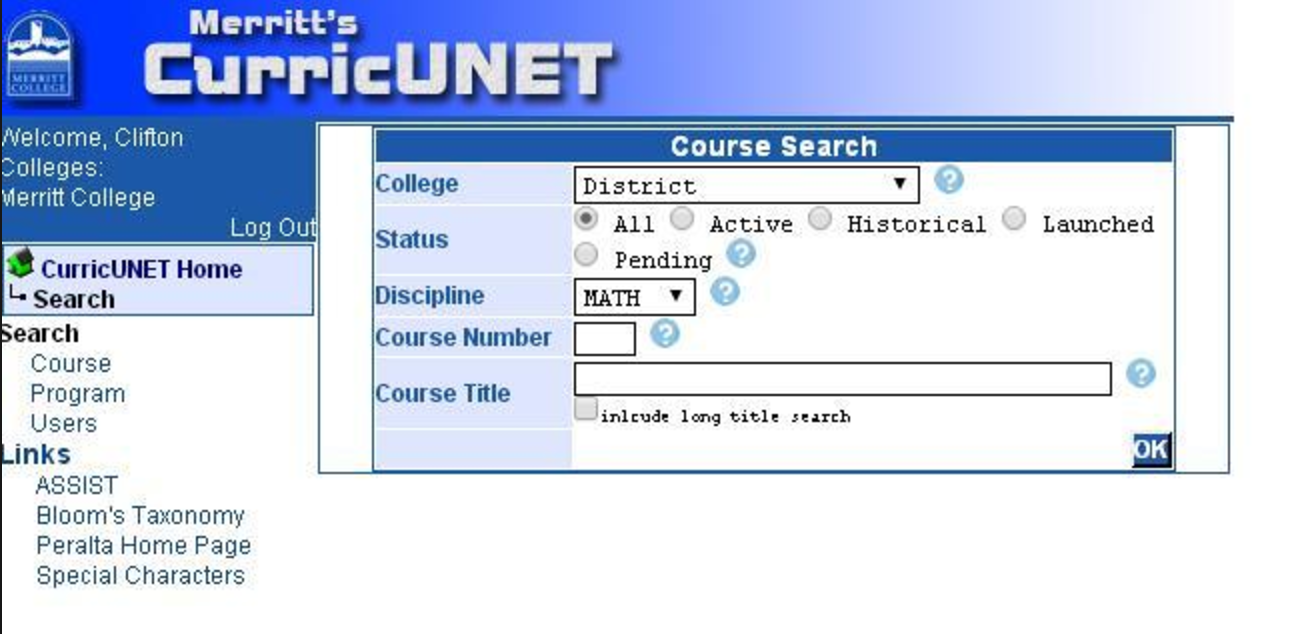
\includegraphics[scale=0.4]{../Figuras/curricunet/curricunet_example}
	\end{figure}
	
\end{frame}

\begin{frame}{Experiencia de usuario}
	\begin{figure}[H]
			\centering
			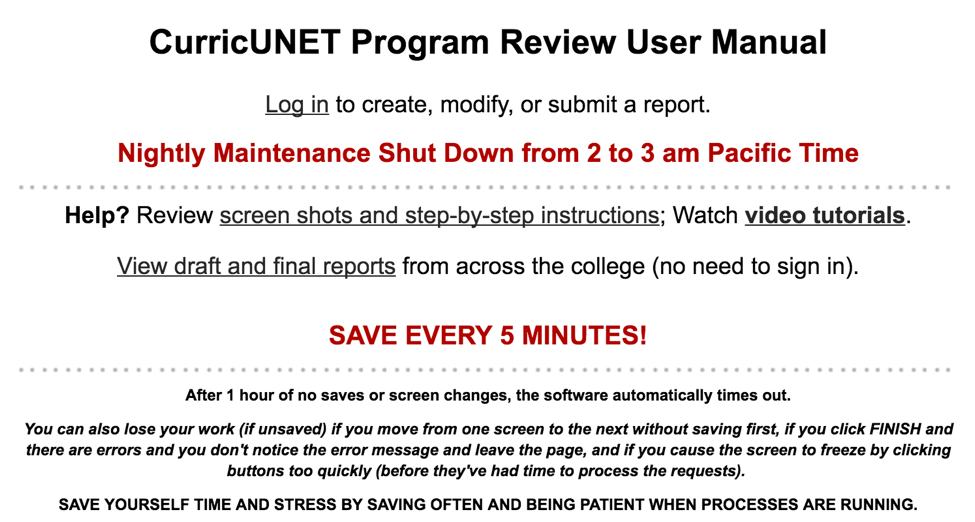
\includegraphics[scale=0.65]{../Figuras/curricunet/curricunet_example_2}
	\end{figure}
	\decoRule \\
  \tiny \textit{$https://www.ccsf.edu/en/employee-services/office-of-instruction/curricunet/curricunet_program_review.html$} \\
\end{frame}

\subsection{Comparación de sistemas relacionados}
\begin{frame}{Comparación de sistemas relacionados}
  	\begin{table}[H]
  	\small
	\centering
	\resizebox{\columnwidth}{!}{%
		\begin{tabular}{lllccl}
		\toprule
		\multicolumn{3}{l}{Características}                                                & CurricUNET                       & CourseLeaf            & DECA         \\
		\midrule
		\rowcolor[HTML]{ECF4FF}
		\multicolumn{3}{l}{Creación y versionamiento de competencias.}                     &                                  &                       &              \\
		\multicolumn{3}{l}{Creación y versionamiento de cursos.}                           & $\checkmark$                     & $\checkmark$          & $\checkmark$ \\
		\multicolumn{3}{l}{Creación y versionamiento de programas de estudio.}             & $\checkmark$                     & $\checkmark$          &              \\
		\multicolumn{3}{l}{Cumple los Estándares de códigos de California.} 			   & $\checkmark$                     &                       &              \\
		\rowcolor[HTML]{ECF4FF}
		\multicolumn{3}{l}{Historial de versiones de competencias.}     			       & 			                      & 		              &  			 \\
		\multicolumn{3}{l}{Historial de versiones de cursos.}     			               & $\checkmark$                     & $\checkmark$          & $\checkmark$ \\
		\multicolumn{3}{l}{Historial de versiones de programas de estudio.}     		   & $\checkmark$                     &  			          & 			 \\
		\multicolumn{3}{l}{Reporte de Comparación entre versiones de cursos.}              & 			                      &                       & $\checkmark$ \\
		\rowcolor[HTML]{ECF4FF}
		\multicolumn{3}{l}{Soporta competencias de aprendizaje del estudiante.}            &                      			  &                       &              \\
		\multicolumn{3}{l}{Plantilla de flujo de trabajo customizable.}                    & $\checkmark$                     &                       &              \\
		\multicolumn{3}{l}{Permite asignar roles evaluadores en la aplicación.}            & $\checkmark$                     & $\checkmark$          &              \\
		\multicolumn{3}{l}{Permite asignar usuarios como colaboradores.}                   & $\checkmark$                     &                       &              \\
		\multicolumn{3}{l}{Soporte de correlatividades entre cursos.}                      & $\checkmark$ 					  &						  &              \\
		\multicolumn{3}{l}{Incluye un catálogo de cursos.}                   		   	   & $\checkmark$					  &	$\checkmark$		  & $\checkmark$ \\
		\multicolumn{3}{l}{Incluye un catálogo de programas de estudio.}                   & $\checkmark$					  &	            		  &              \\
		\rowcolor[HTML]{ECF4FF}
		\multicolumn{3}{l}{Incluye un catálogo de competencias.}                   	       & 								  &						  & 			 \\
		\multicolumn{3}{l}{UX intuitiva y efectiva.}     			   					   &                                  & $\checkmark$          & $\checkmark$ \\
		\bottomrule
		\end{tabular}
	}
	\end{table}
\end{frame}

% Requisitos no claros
\subsection{Problemática}
\begin{frame}{Problemática}
	\begin{columns}[c,onlytextwidth]
    	\column{0.6\textwidth}
		\begin{block}{}
			\begin{itemize}
	        	\item Sistemas actuales utilizan tecnología atrasada.
				\item Confusa experiencia de usuario.
				\item Falta de integracion con sistemas de administración de competencias.
				\item Requerimientos cambiantes.
	    	\end{itemize}
		\end{block}
	    \column{0.4\textwidth}
		\begin{figure}[H]
			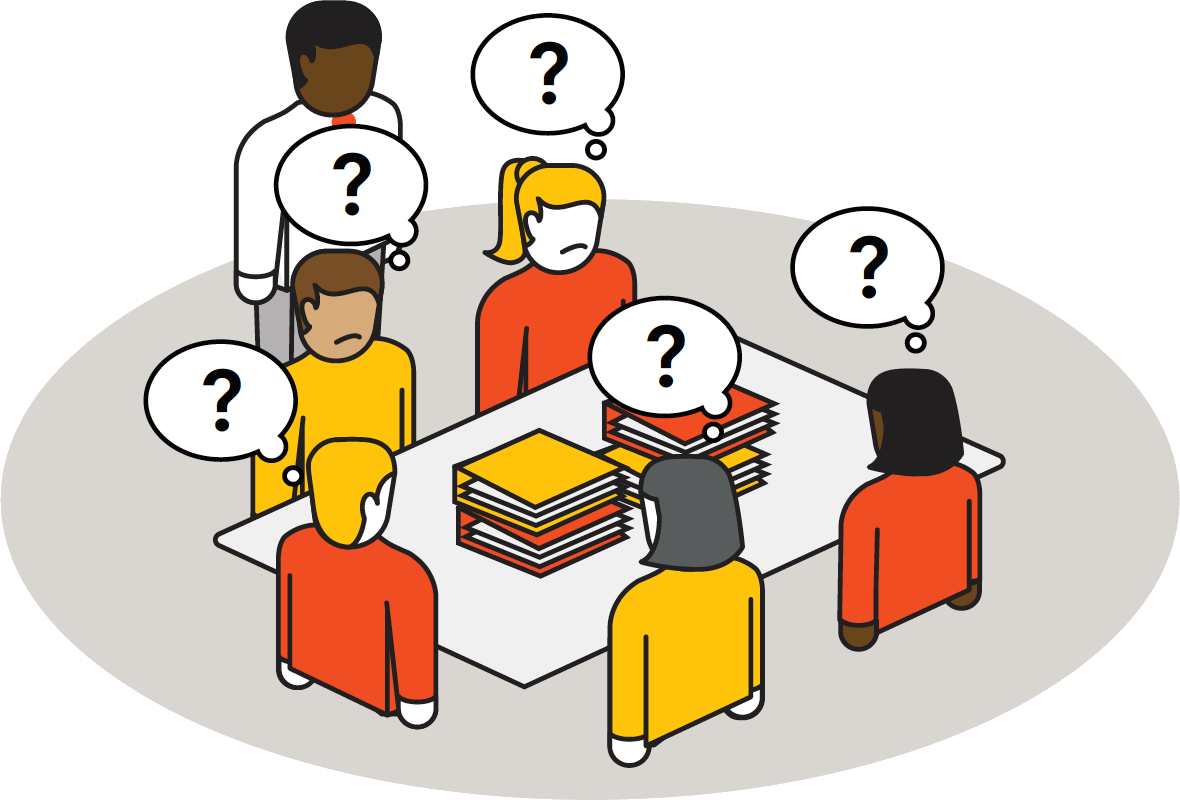
\includegraphics[scale=0.2]{../Figuras/unhappy_agile}
		\end{figure}
  	\end{columns}
\end{frame}

% OBJETIVOS
\section{Objetivos}
\subsection{Objectivo General}
\begin{frame}[t]{Objetivos}
	\metroset{block=fill}
	\begin{alertblock}{Objetivo general}
        Diseñar una aplicación que permita integrar y estructurar tareas separadas de un sistema académico para una gestión de programas educativos orientados a resultados pedagógicos, que provea soporte a flujos de trabajo para sus diferentes etapas de aprobación.
      \end{alertblock}
\end{frame}

\subsection{Objetivos específicos}
\begin{frame}[t]{Objetivos}
	\metroset{block=fill}
	\begin{alertblock}{Objetivo general}
        Diseñar una aplicación que permita integrar y estructurar tareas separadas de un sistema académico para una gestión de programas educativos orientados a resultados pedagógicos, que provea soporte a flujos de trabajo para sus diferentes etapas de aprobación.
      \end{alertblock}

	\metroset{block=fill}
	\begin{alertblock}{Objetivos específicos}
        \begin{itemize}
        	\item Realizar un relevamiento de los requerimientos, diseño e implementación de un sistema de gestión de programas orientado a competencias.
        	\item Realizar el proyecto en un marco de programación ágil, estimando y desarrollando la aplicación de acuerdo a las directrices brindadas por la metodología.
        	\item Validar la herramienta desarrollada: con expertos del dominio principalmente y de manera preliminar con experiencias limitadas con los usuarios finales.
        \end{itemize}
    \end{alertblock}
\end{frame}

% PROPUESTA DE TRABAJO
\section{Propuesta de trabajo}
\subsection{Caso de estudio}
\begin{frame}{Caso de estudio}
  	Caso de estudio de observación participante: desarrollo de un sistema de curriculums orientado a competencias.

	\begin{block}{Requerimientos no funcionales}
		\begin{itemize}
        	\item Aplicación web.
			\item SaaS.
			\item Utilización de abordaje ágil de desarrollo.
    	\end{itemize}
	\end{block}

\end{frame}

\subsection{Flujo de trabajo durante el desarrollo}
\begin{frame}{Flujo de trabajo durante el desarrollo}
	\begin{figure}
		\centering
	    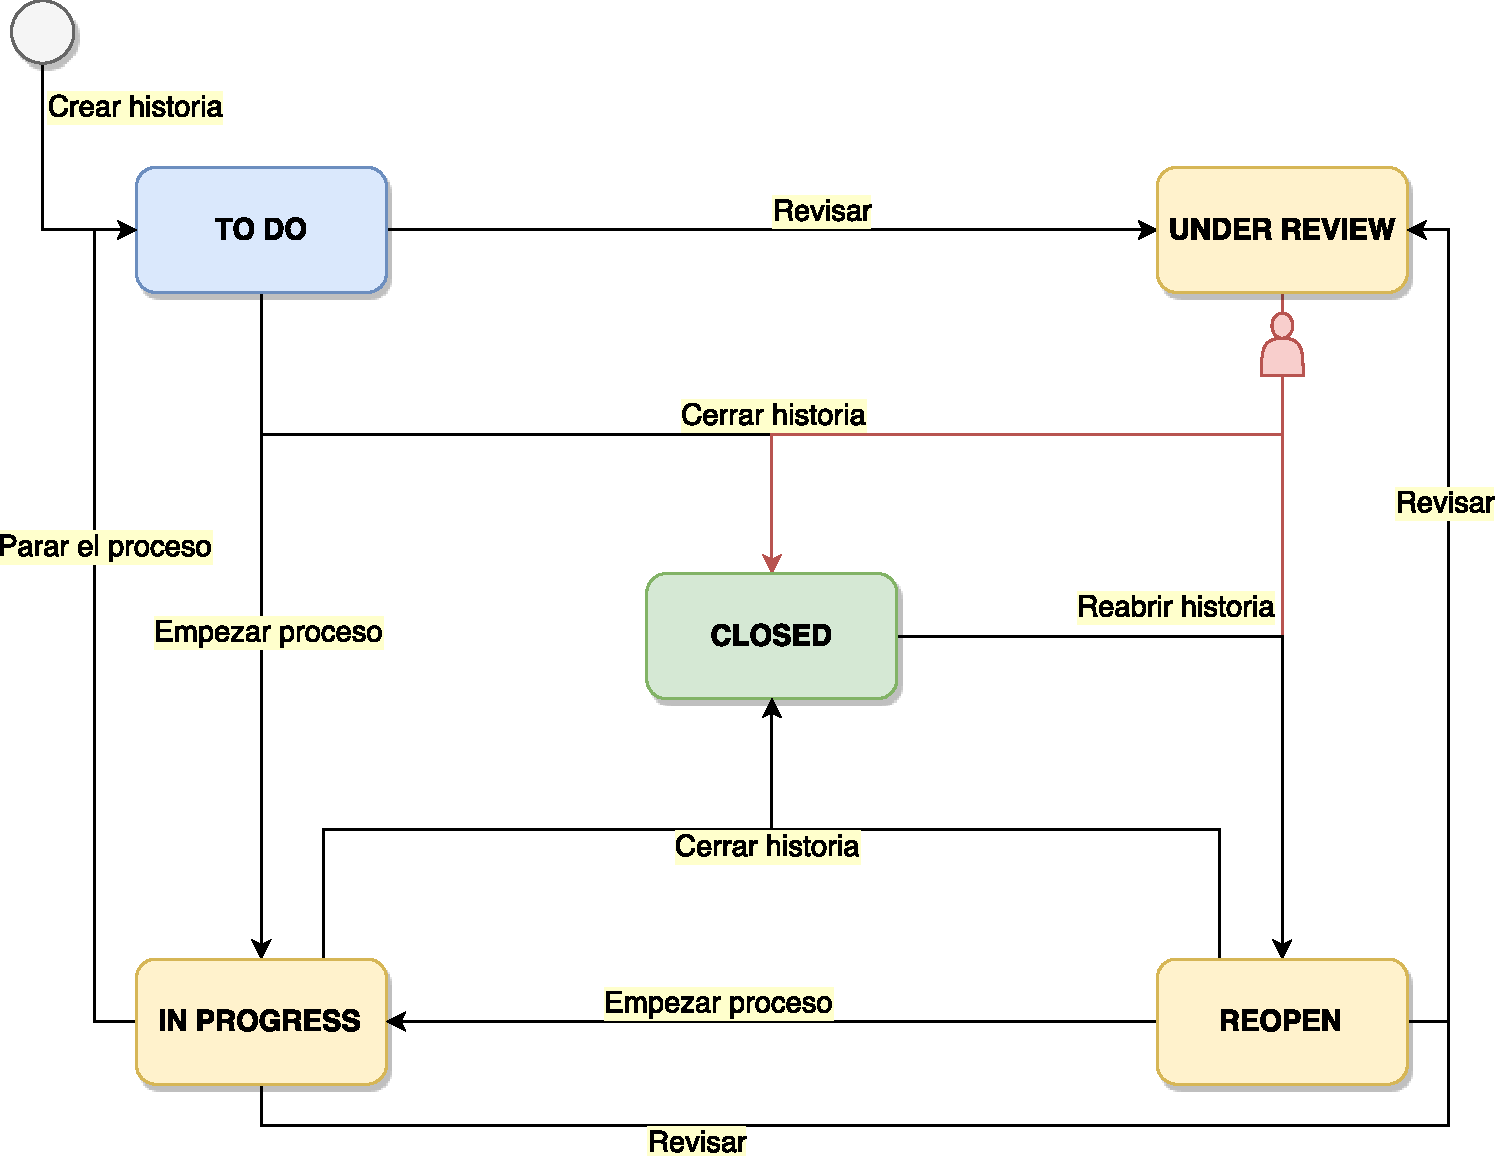
\includegraphics[scale=0.35]{../Figuras/workflow}
	\end{figure}
\end{frame}

% MARCO TEORICO
\section{Estado del arte}
\subsection{Aplicaciones web}
\begin{frame}{Aplicaciones web}
	\metroset{block=fill}
	\begin{alertblock}{Definición}
		Software con arquitectura cliente-servidor donde el cliente corre por lo general en un navegador web.
	\end{alertblock}
	\begin{columns}[c,onlytextwidth]
    	\column{0.6\textwidth}
		\begin{block}{Características}
			\begin{itemize}
	        	\item Ubicuidad.
	        	\item Bajos requerimientos en Hardware.
	        	\item Actualizaciones inmediatas.
	        	\item No requiere instalaciones.
	    	\end{itemize}
		\end{block}
	    \column{0.4\textwidth}
		\begin{figure}[H]
			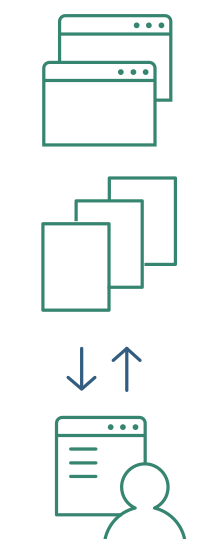
\includegraphics[scale=0.23]{../Figuras/web_app}
		\end{figure}
  	\end{columns}
\end{frame}

\subsection{Cloud Computing}
\begin{frame}{Cloud Computing}
	\metroset{block=fill}
	\begin{alertblock}{Definición}
		Metáfora de abastecimiento y consumición de recursos de infraestructura.
	\end{alertblock}

	\begin{columns}[c,onlytextwidth]
    	\column{0.6\textwidth}
		\begin{block}{Características}
			\begin{itemize}
	        	\item Servicios a demanda.
	        	\item Disposición de recursos.
	        	\item Informes de uso de servicios.
	        	\item Escalabilidad.
	      		\item Amplio acceso de red.
	    	\end{itemize}
		\end{block}
	    \column{0.4\textwidth}
		\begin{figure}[H]
			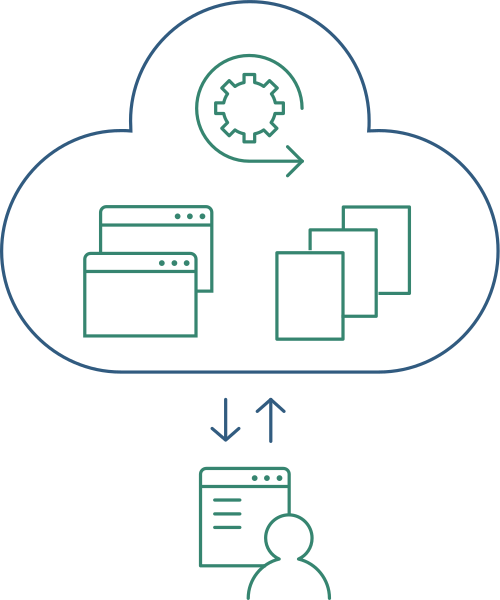
\includegraphics[scale=0.23]{../Figuras/cloud_computing}
		\end{figure}
  	\end{columns}
\end{frame}

\subsection{Software as a service}
\begin{frame}{Software as a service}
	\metroset{block=fill}
	\begin{alertblock}{Definición}
		Paradigma de entrega de software como servicio a través de una red.
	\end{alertblock}

	\begin{columns}[c,onlytextwidth]
    	\column{0.6\textwidth}
		\begin{block}{Características}
			\begin{itemize}
	        	\item Modelo de suscripción.
	        	\item Acceso y administración a través de una red.
	        	\item Actividades gestionadas desde ubicaciones centrales.
	        	\item Actualizaciones centralizadas.
	      		\item Arquitectura multi-tenant.
	    	\end{itemize}
		\end{block}
	    \column{0.4\textwidth}
		\begin{figure}[H]
			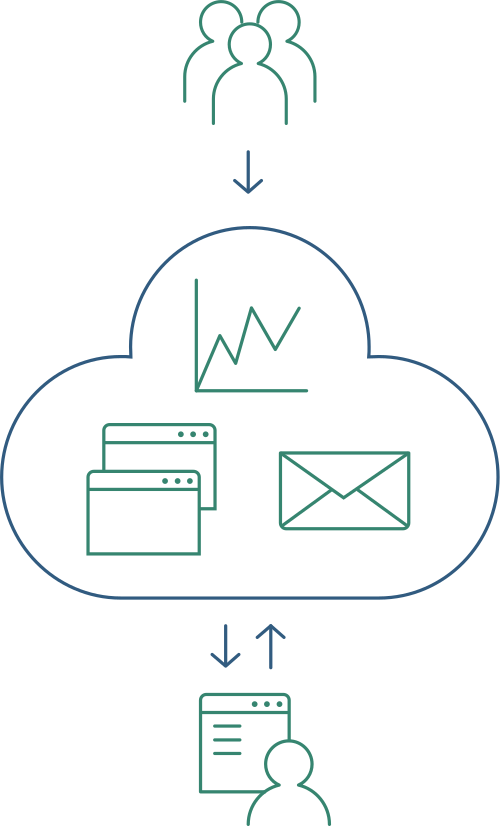
\includegraphics[scale=0.23]{../Figuras/saas}
		\end{figure}
  	\end{columns}
\end{frame}

\subsection{Sistemas de gestión de evaluaciones basadas en competencias}
\begin{frame}{Sistemas de gestión de evaluaciones basadas en competencias}
	\begin{figure}
		\centering
	    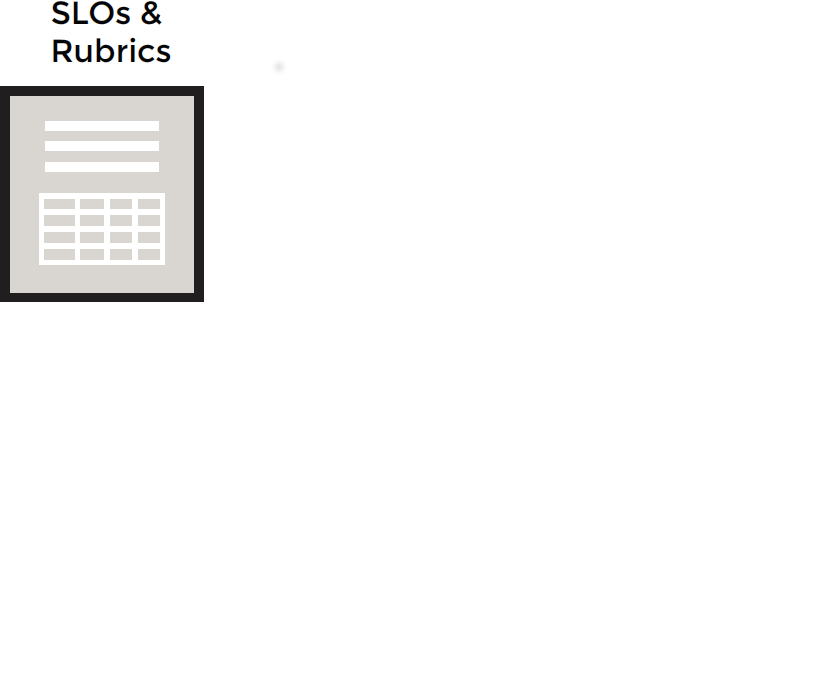
\includegraphics[scale=0.55]{../Figuras/ams/ams_1}
	\end{figure}
\end{frame}

\begin{frame}{Gestión de evaluaciones basadas en competencias}
	\begin{figure}
		\centering
	    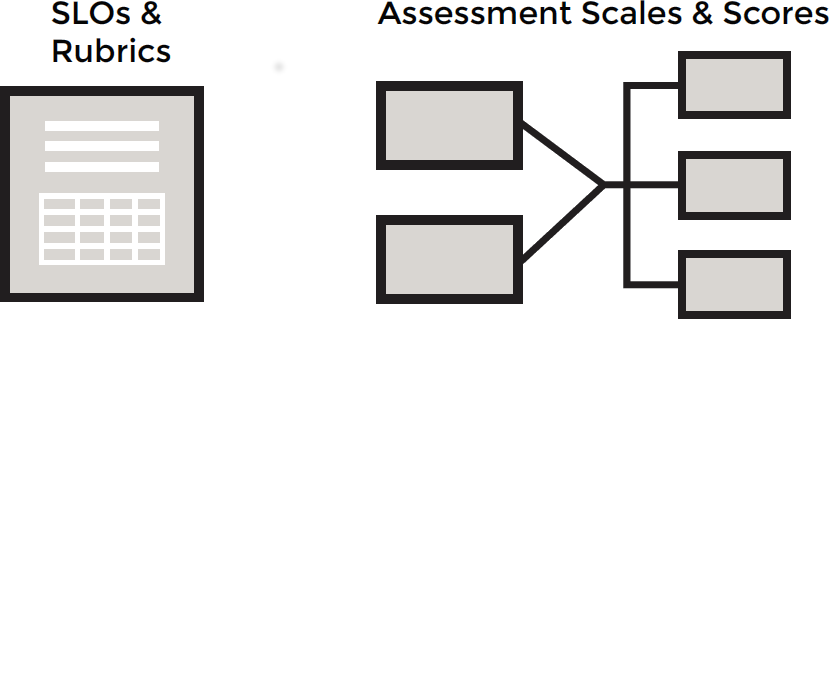
\includegraphics[scale=0.55]{../Figuras/ams/ams_2}
	\end{figure}
\end{frame}

\begin{frame}{Gestión de evaluaciones basadas en competencias}
	\begin{figure}
		\centering
	    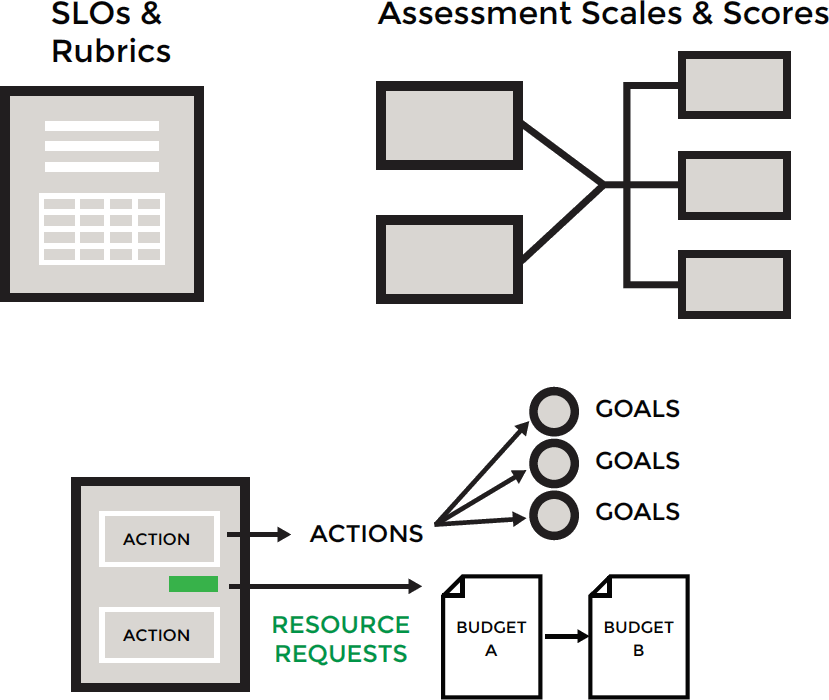
\includegraphics[scale=0.55]{../Figuras/ams/ams_3}
	\end{figure}
\end{frame}

\subsection{Metodología ágil}
\begin{frame}{Metodología ágil}
	\metroset{block=fill}
	\begin{alertblock}{Definición}
		Enfoque para toma de decisiones basado en el desarrollo iterativo e incremental.
	\end{alertblock}

	\begin{columns}[c,onlytextwidth]
    	\column{0.5\textwidth}
		\begin{block}{Características}
			\begin{itemize}
	        	\item Entregas de valor agregado en iteraciones.
	        	\item Adaptación al cambio.
	        	\item El cliente es parte del proceso de desarrollo.
	    	\end{itemize}
		\end{block}
	    \column{0.5\textwidth}
		\begin{figure}
		    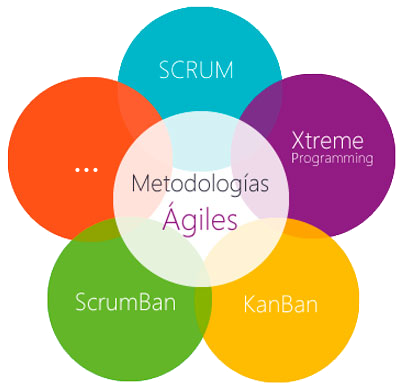
\includegraphics[scale=0.32]{../Figuras/met_agiles}
		\end{figure}
  	\end{columns}
\end{frame}

\section{Métricas de éxito}
\subsection{UserVoice}
\begin{frame}{UserVoice}
	\begin{figure}
		\centering
	    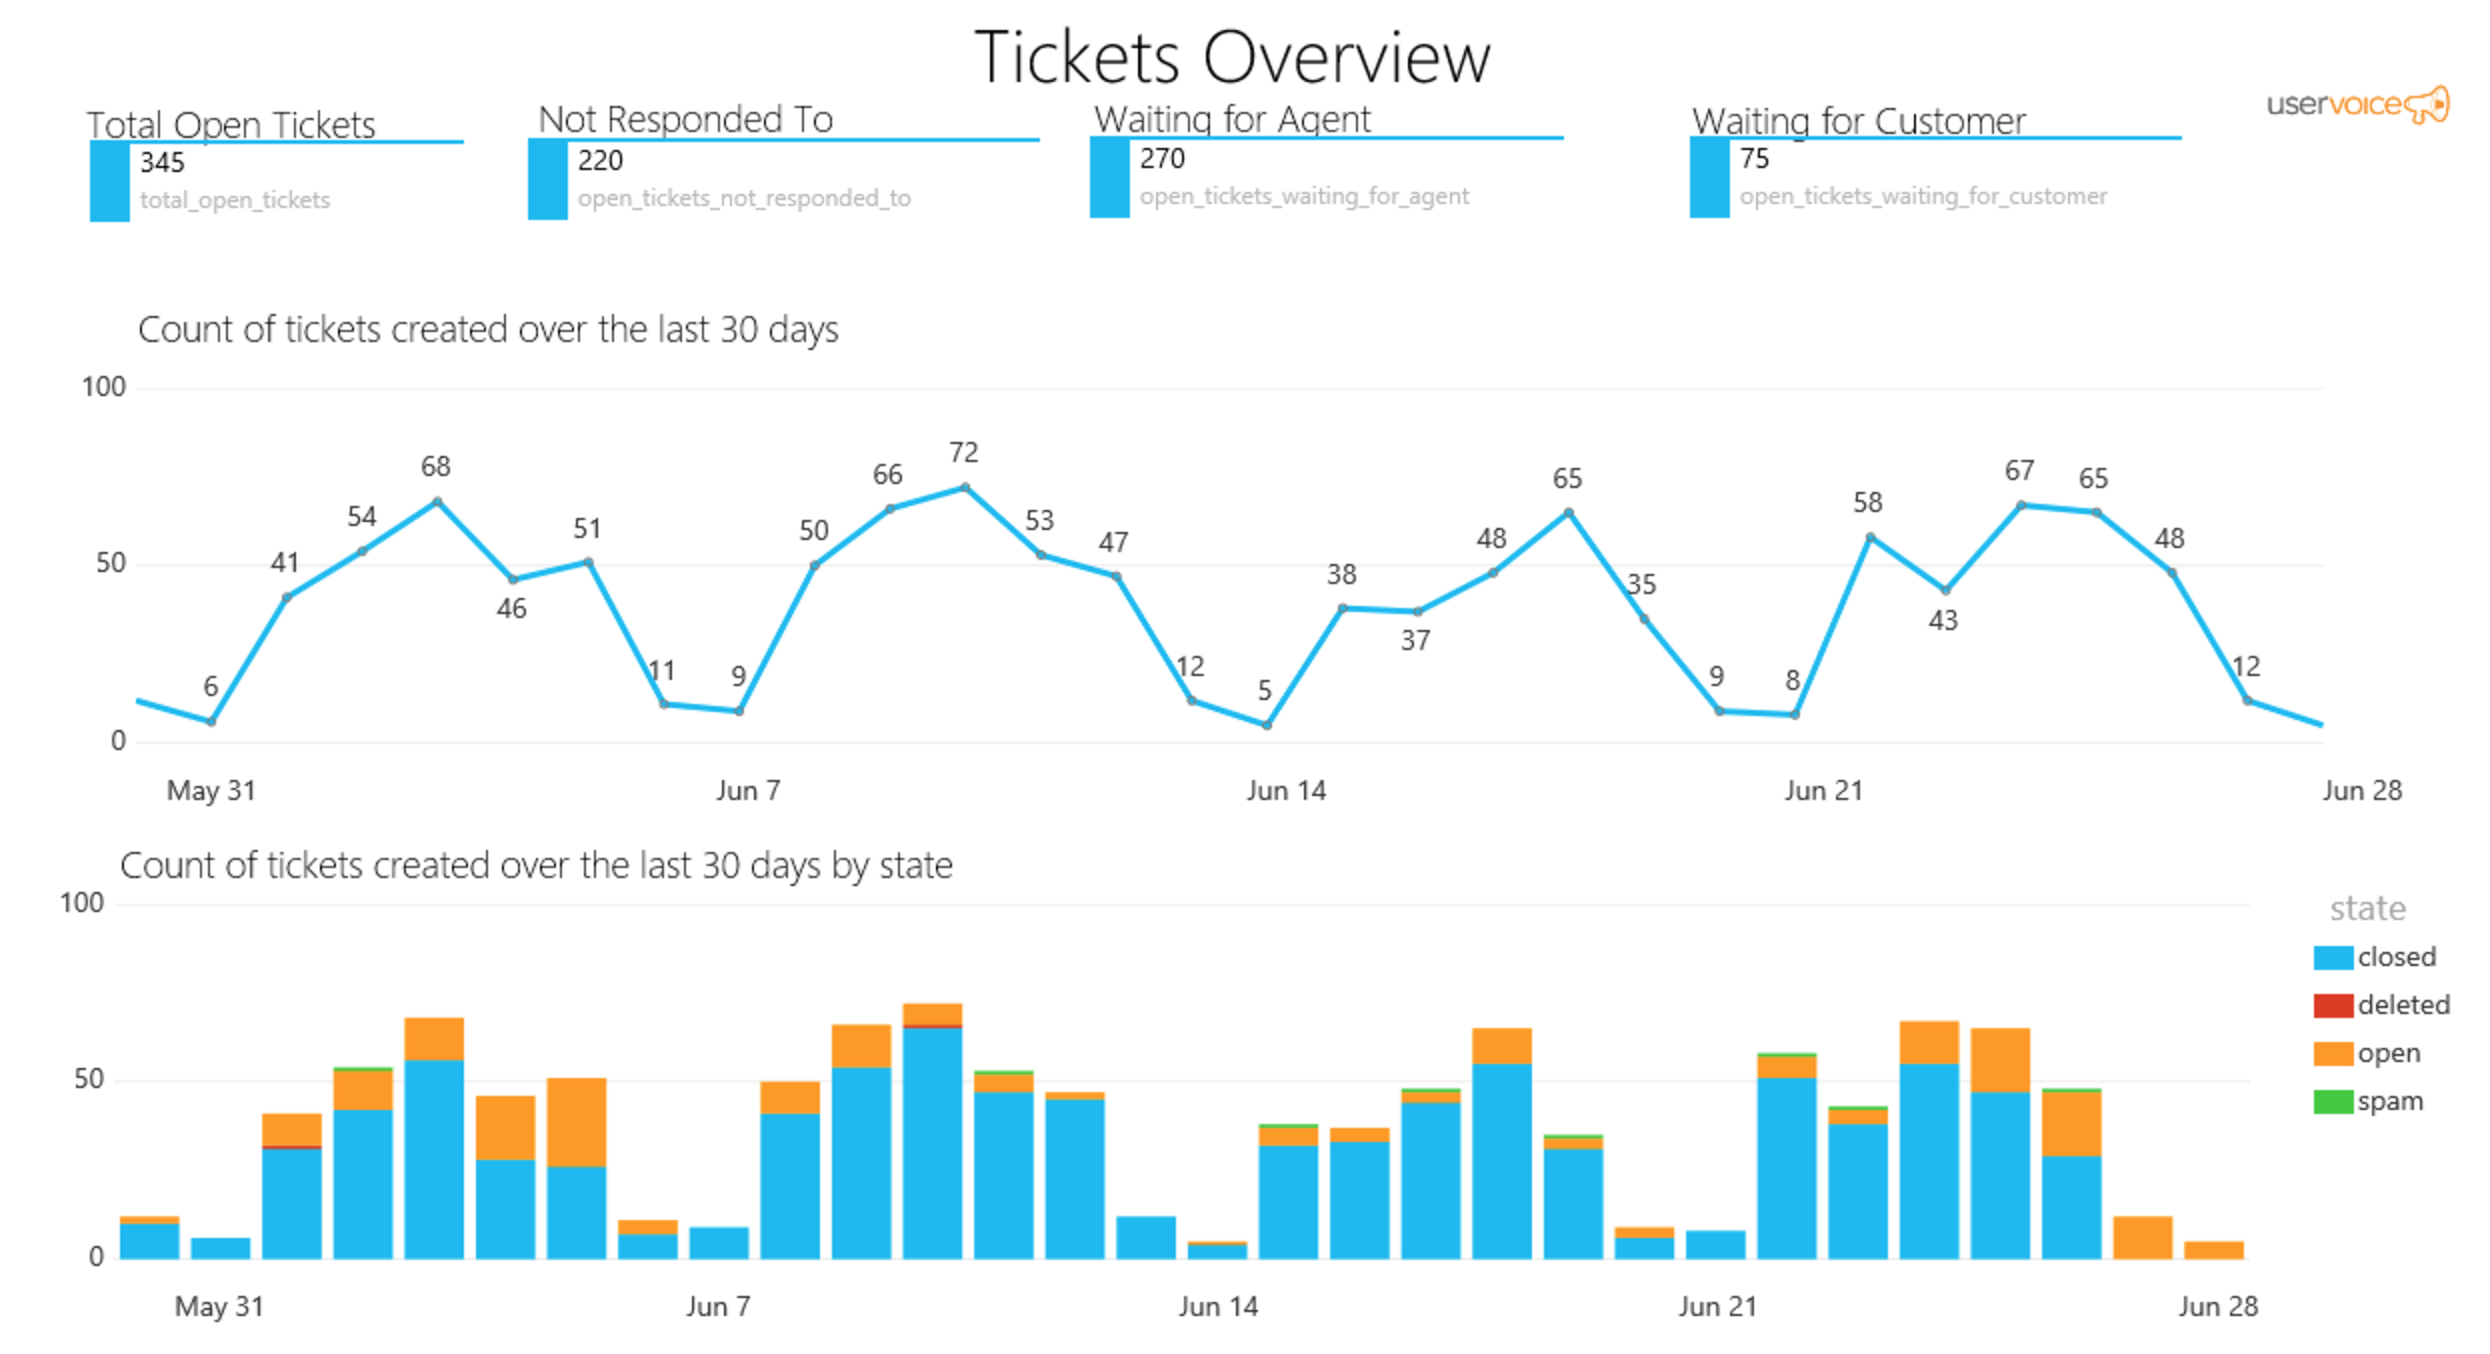
\includegraphics[scale=0.25]{../Figuras/metricas/uservoice}
	\end{figure}
\end{frame}

% CONCLUSIONES Y TRABAJOS FUTUROS
\section{Proceso de implementación}
\subsection{Experiencia de usuario}
\begin{frame}{Experiencia de usuario}
	\begin{figure}[H]
		\centering
		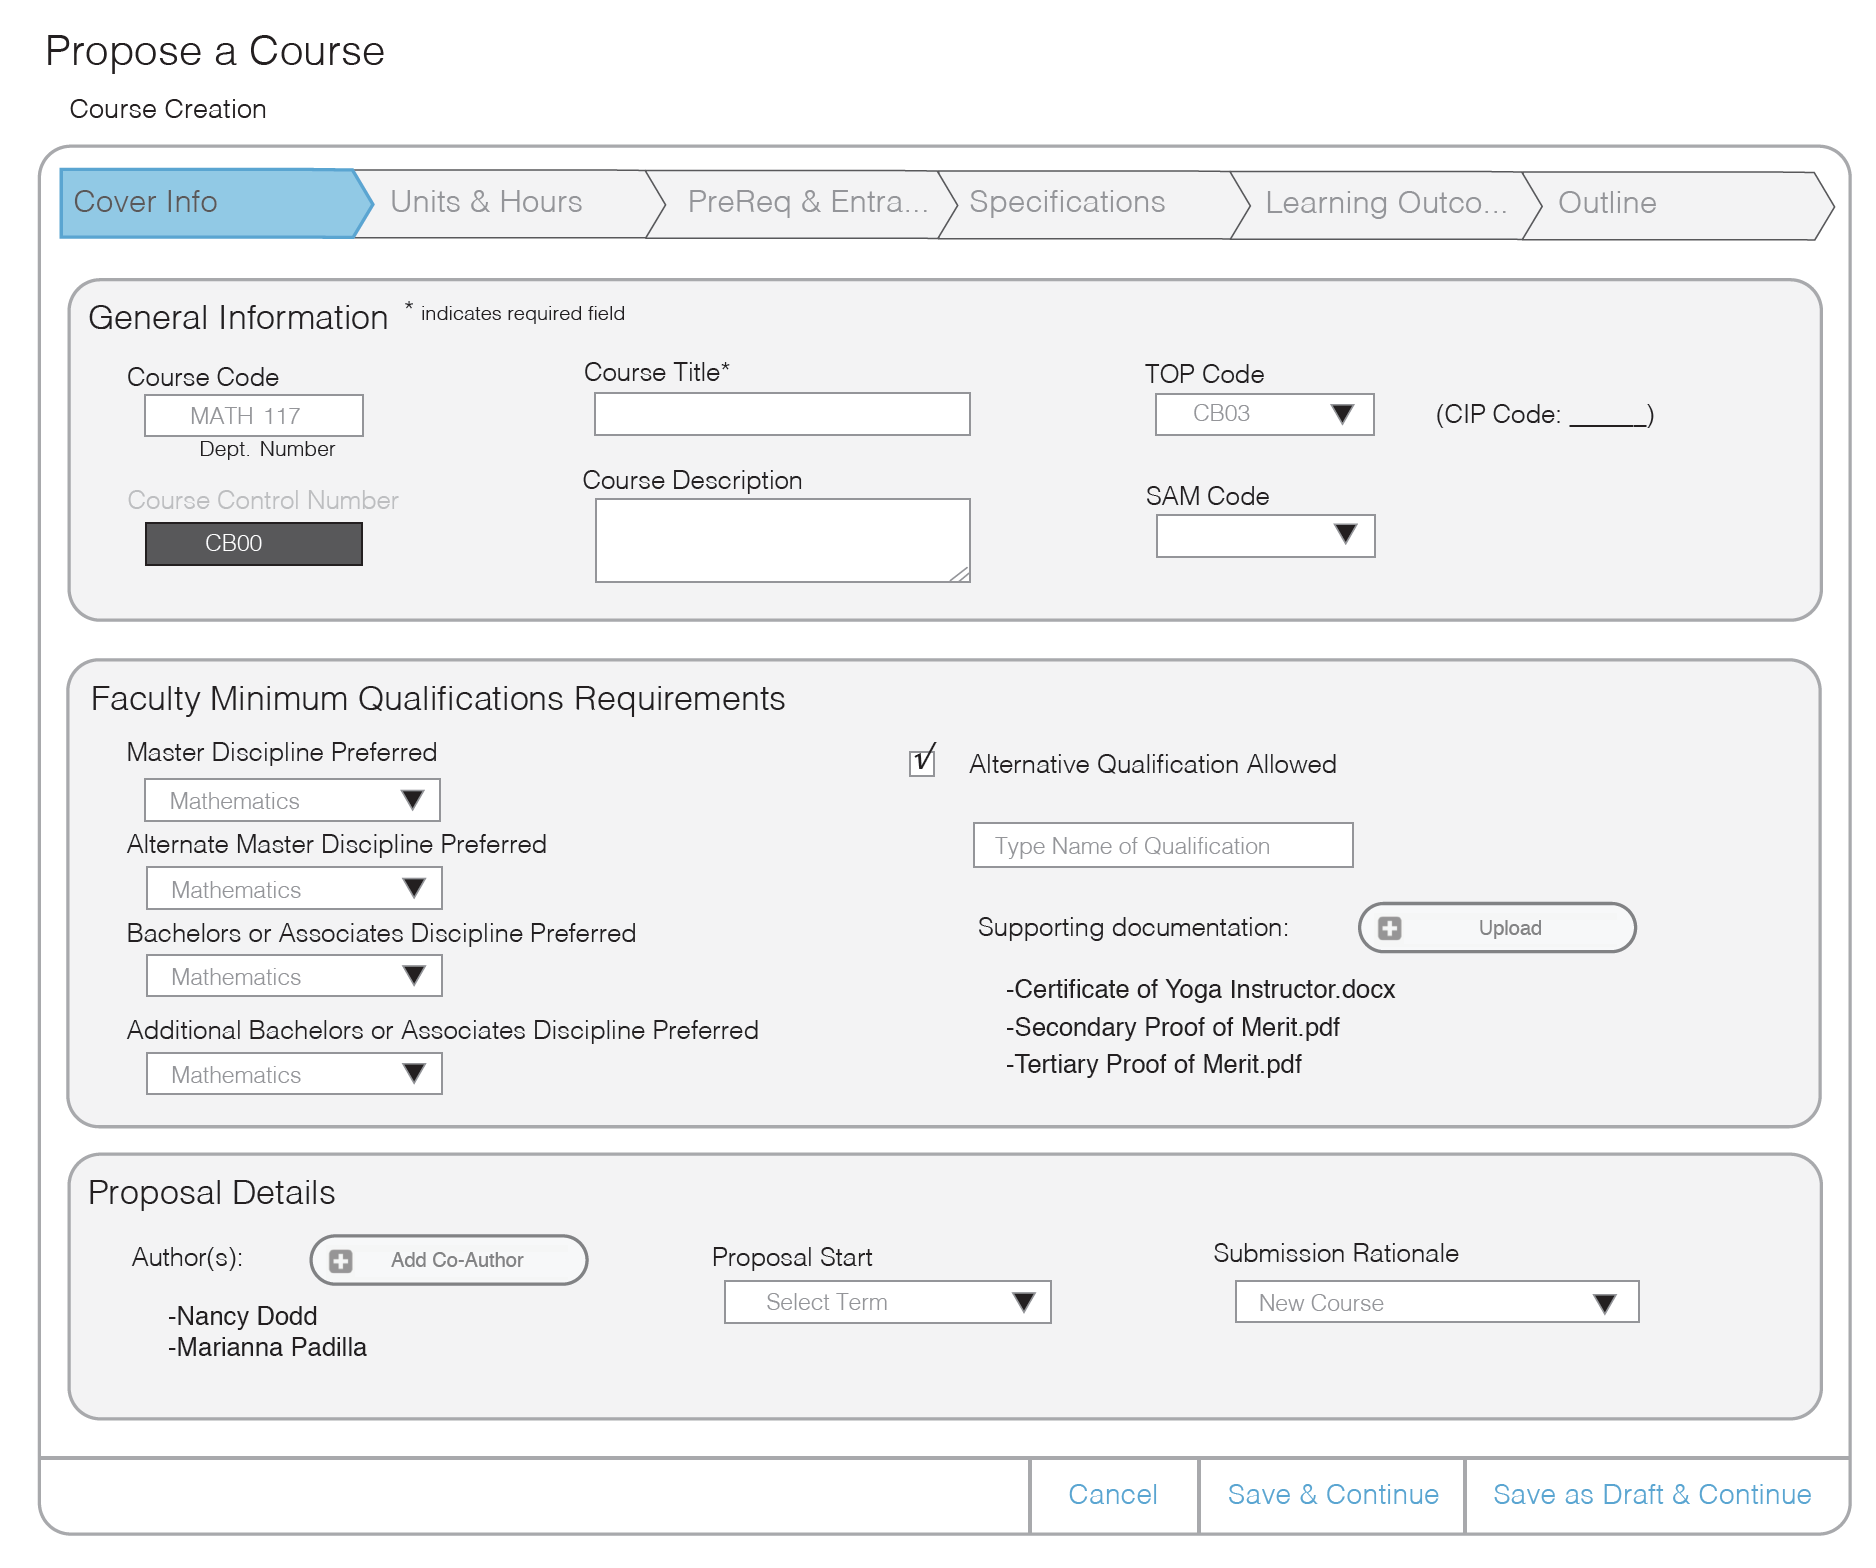
\includegraphics[scale=0.25]{../Figuras/mockups/el_curr_2}
	\end{figure}
\end{frame}

\begin{frame}{Experiencia de usuario}
	\begin{figure}[H]
		\centering
		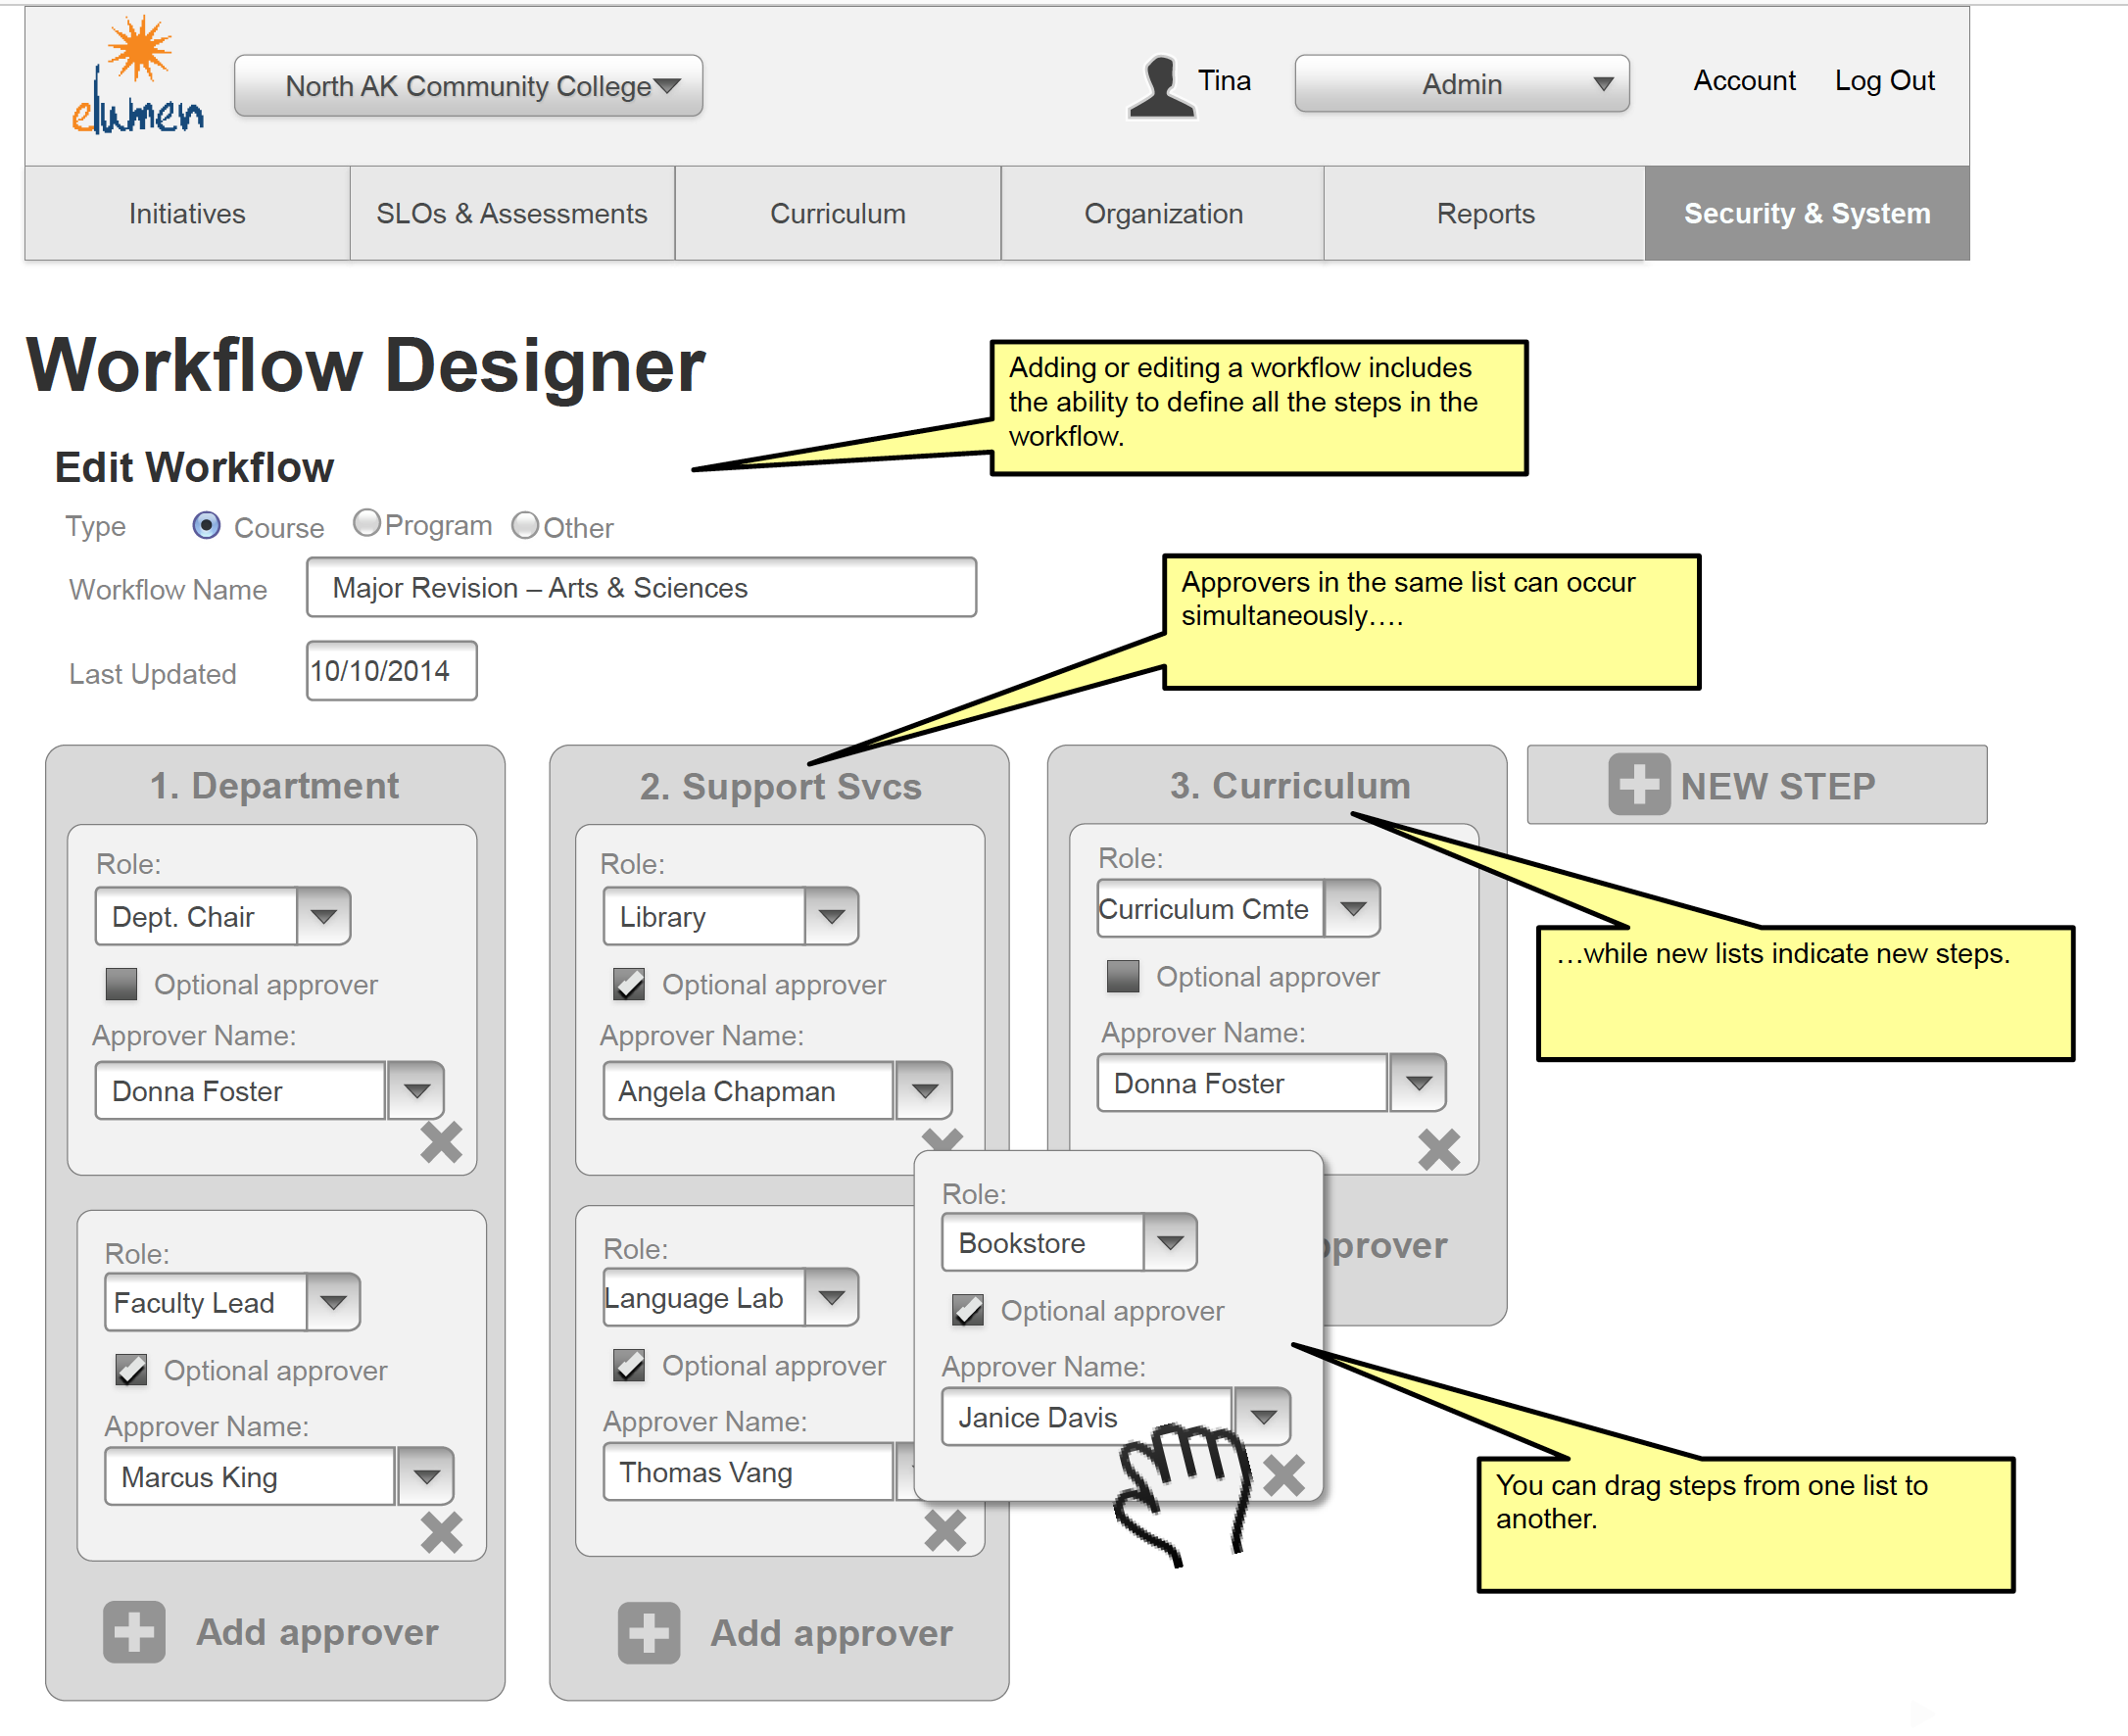
\includegraphics[scale=0.24]{../Figuras/mockups/el_curr_1}
	\end{figure}
\end{frame}

\subsection{Módulo curricular integrado a competencias}
\begin{frame}{Módulo curricular integrado a competencias}
	\begin{figure}
		\centering
	    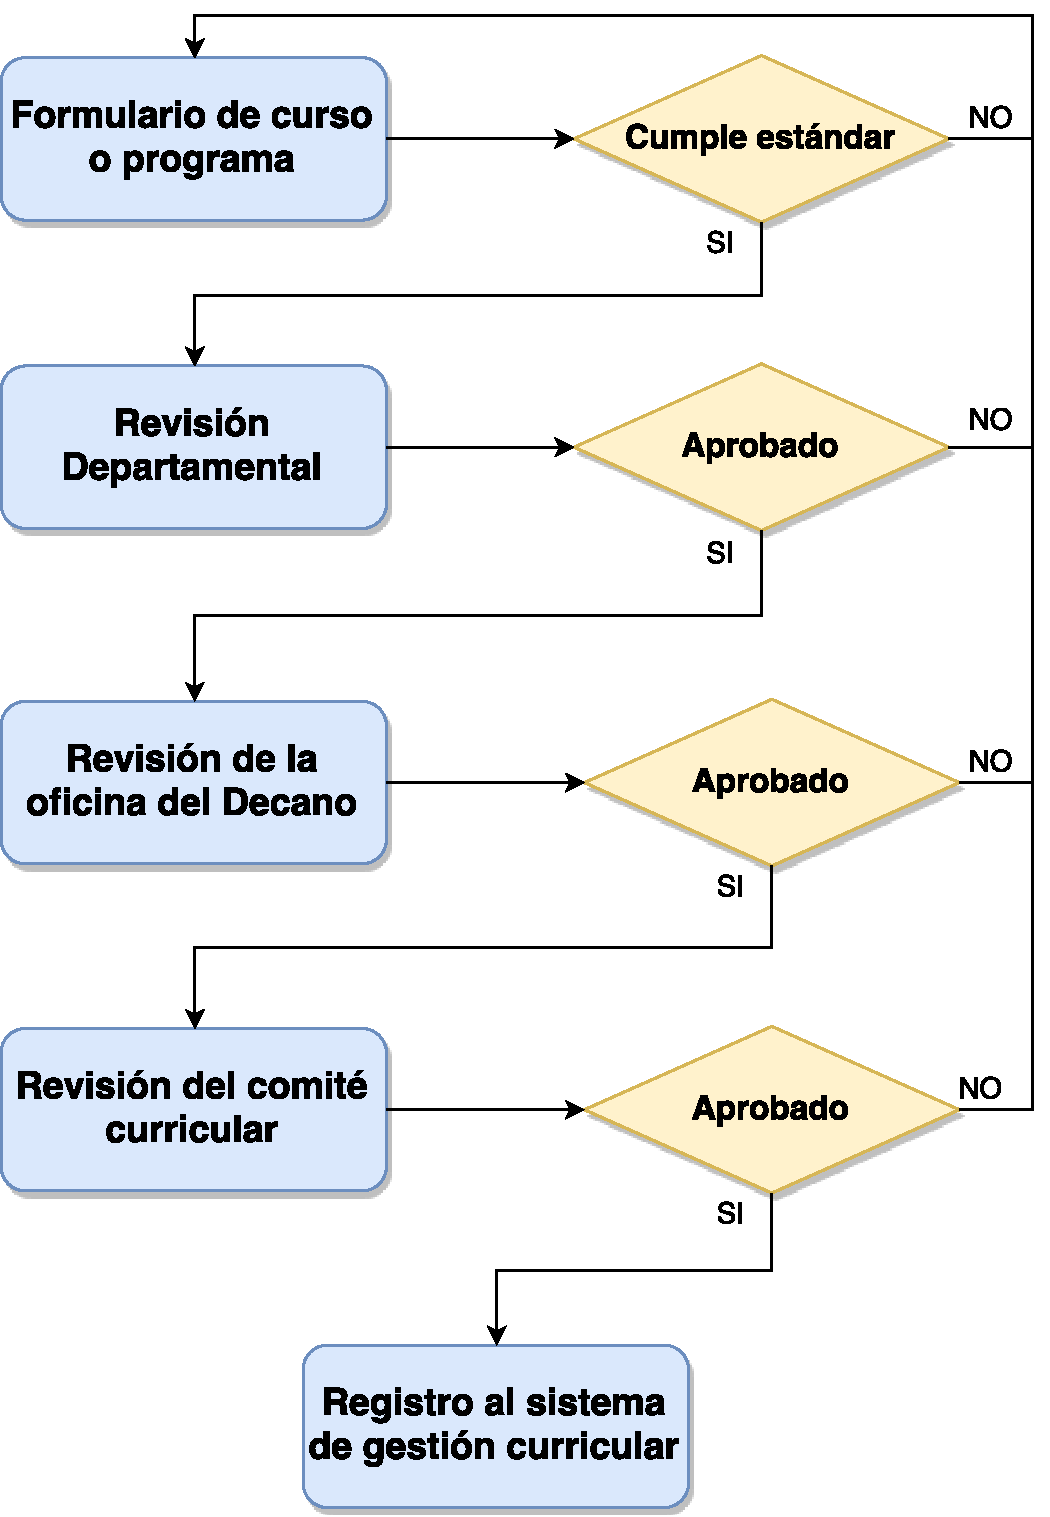
\includegraphics[scale=0.25,left]{../Figuras/problematica/course_creation_flow}
	\end{figure}
\end{frame}

\subsection{Módulo de gestión curricular integrado a un sistema de gestión de competencias}
\begin{frame}{Módulo curricular integrado a competencias}
	\begin{figure}
		\centering
	    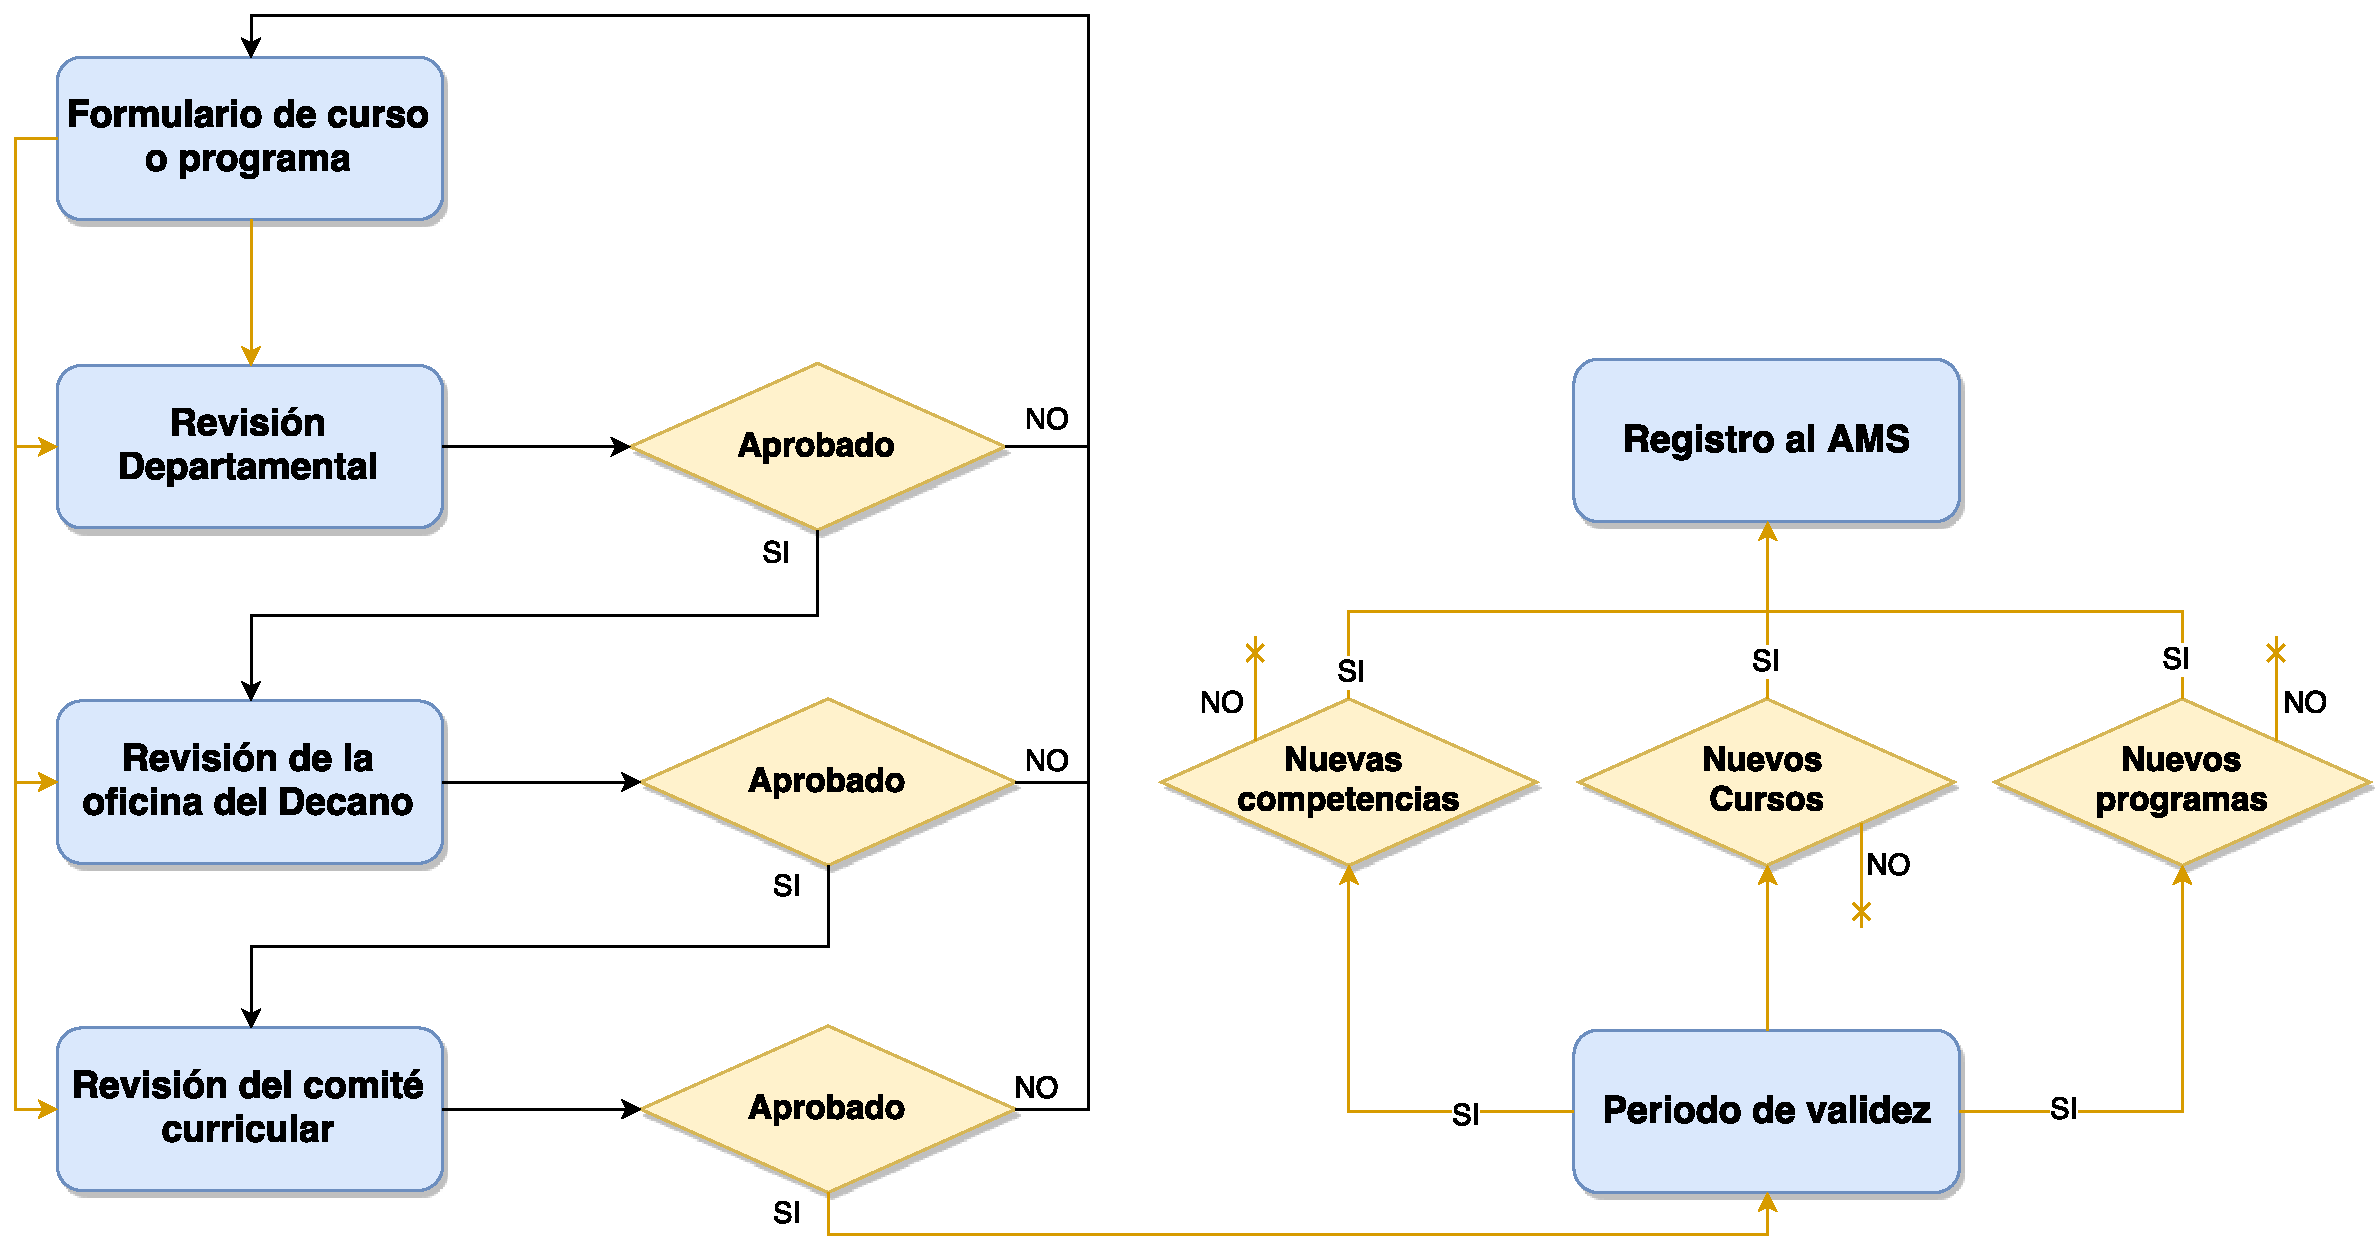
\includegraphics[scale=0.25,left]{../Figuras/propuesta/proposal}
	\end{figure}
\end{frame}

\begin{frame}{Modelo de la propuesta de solución}
	\begin{figure}
		\centering
	    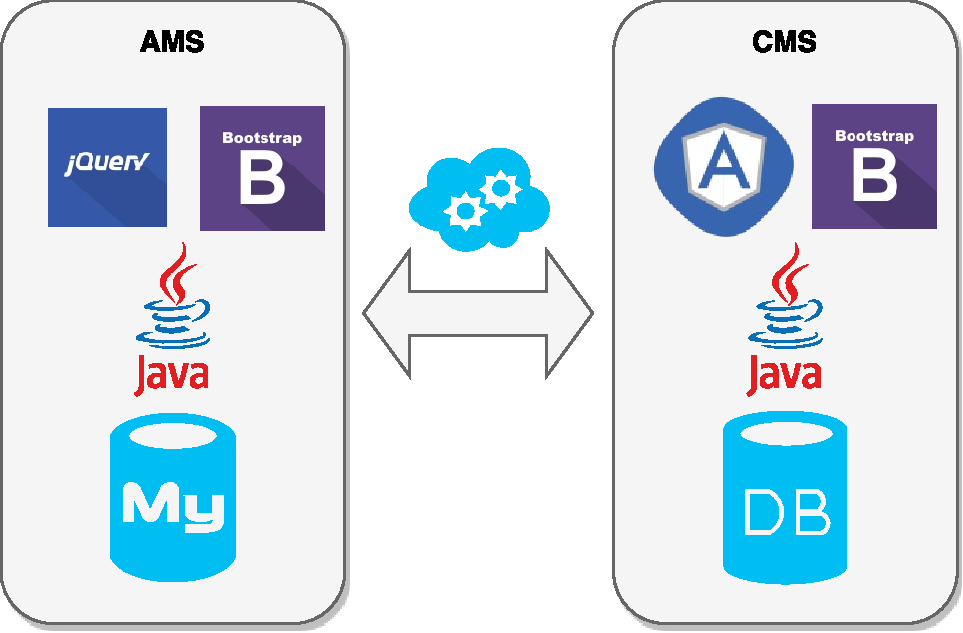
\includegraphics[scale=0.55]{../Figuras/propuesta/architecture}
	\end{figure}
\end{frame}

\section{Trabajo realizados y futuros}
\subsection{Diagrama de trabajos}
\begin{frame}{Diagrama de trabajos}
	\begin{figure}
		\centering
	    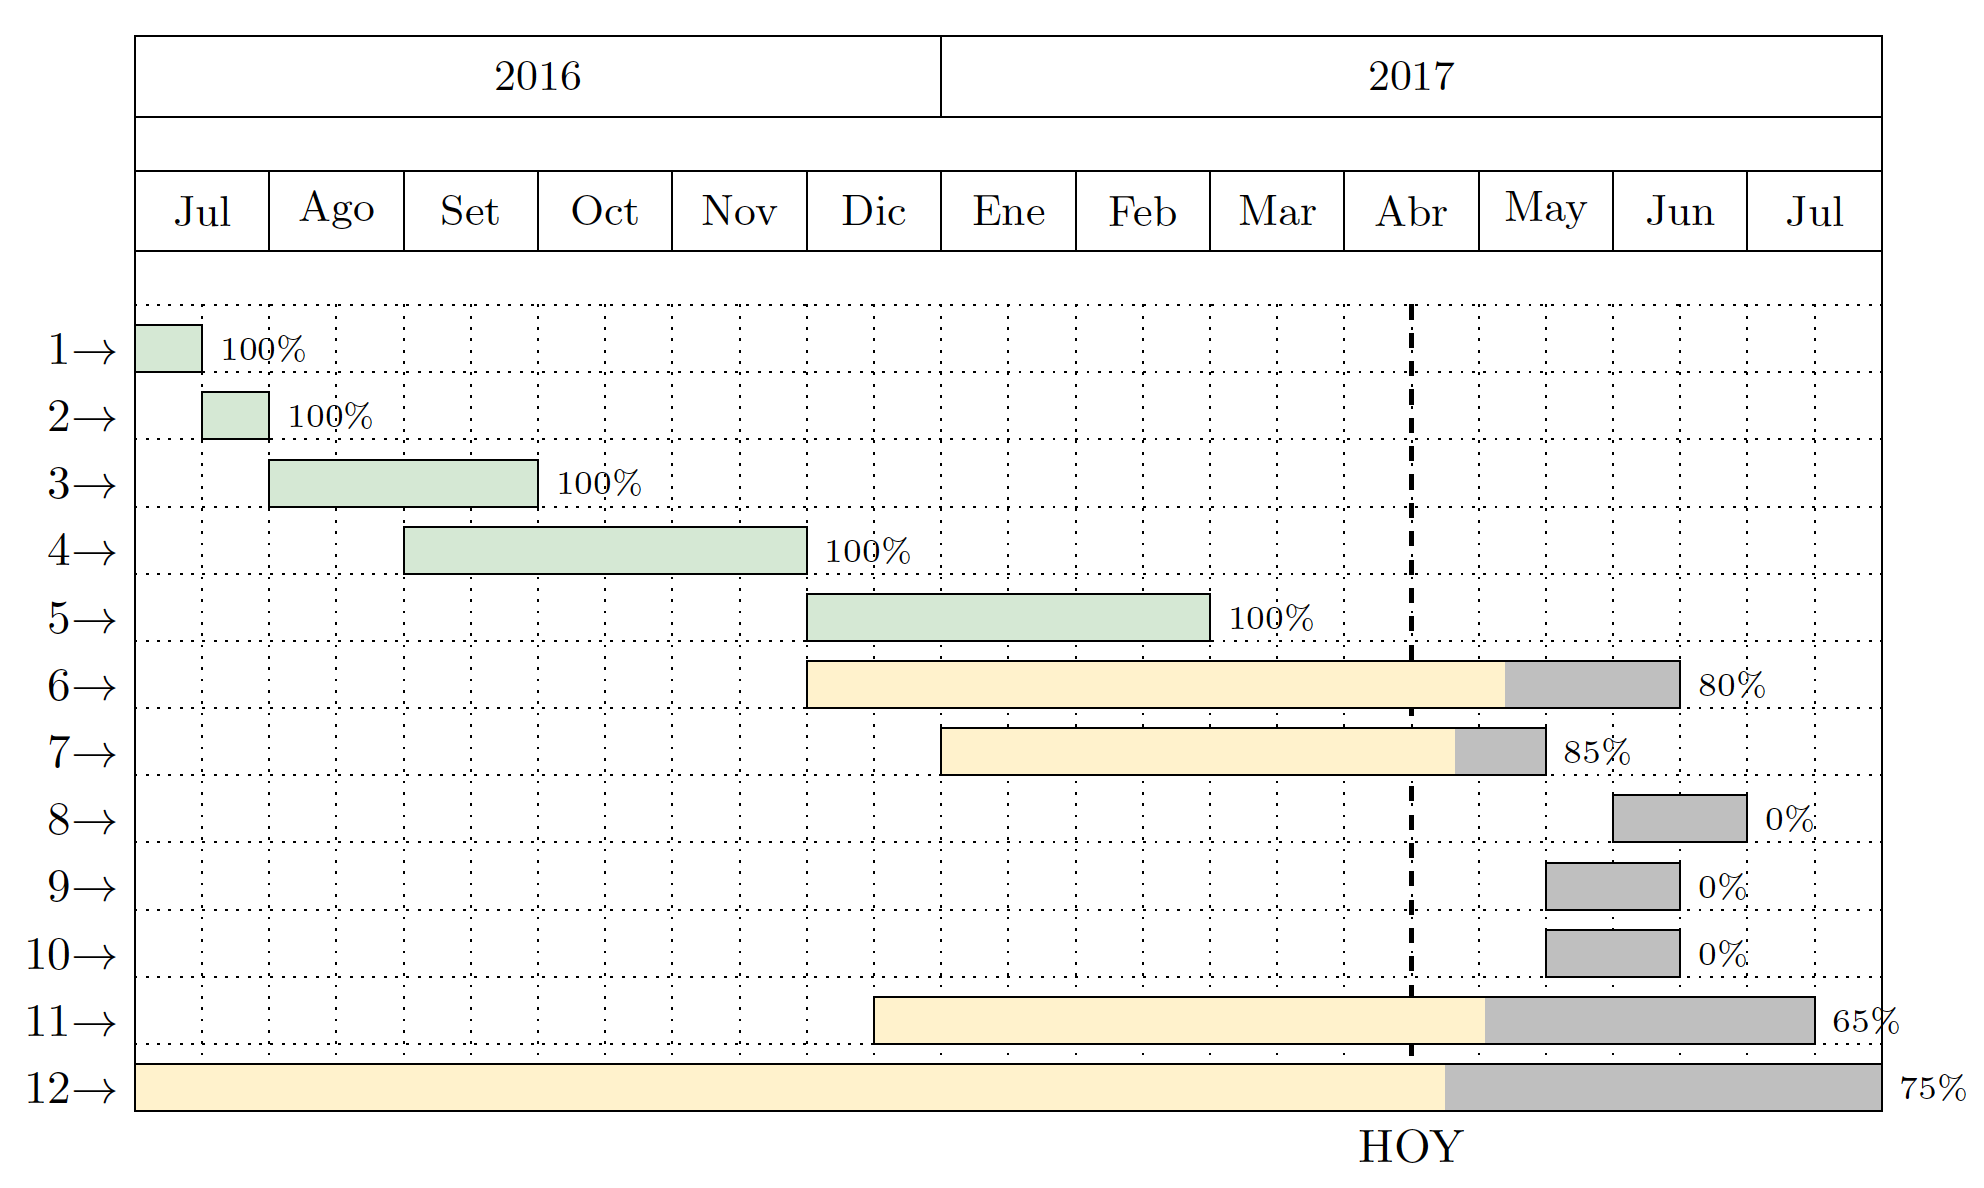
\includegraphics[scale=0.3]{../Figuras/proceso/gantt}
	\end{figure}
\end{frame}

\begin{frame}[standout]
  ¡Gracias por su atención!
\end{frame}


\end{document}
